%%%%%%%%%%%%%%%%%%%%%%%%%%%%%%%%%%%%%%%%%%%%%%%%%%%%%%%%%%%%%%%%%%%%%%
%%  Copyright by Wenliang Du.                                       %%
%%  This work is licensed under the Creative Commons                %%
%%  Attribution-NonCommercial-ShareAlike 4.0 International License. %%
%%  To view a copy of this license, visit                           %%
%%  http://creativecommons.org/licenses/by-nc-sa/4.0/.              %%
%%%%%%%%%%%%%%%%%%%%%%%%%%%%%%%%%%%%%%%%%%%%%%%%%%%%%%%%%%%%%%%%%%%%%%

\newcommand{\commonfolder}{../../common-files}
\input{\commonfolder/header}

%% Chinese versions of the user-visible common macros.
\renewcommand{\seedsubmission}{你需要提交一份详细的实验报告，并附上截图，
用来说明你完成了什么、观察到了什么。对于有趣或出乎意料的观察结果，
你还需要给出解释。请同时列出重要的代码片段，并对这些代码进行解释。
只提交代码而没有解释将不会获得分数。}

\renewcommand{\seedbook}{\textit{Computer \& Internet Security: A Hands-on Approach}，
第 3 版，Wenliang Du 著。详情见 \url{https://www.handsonsecurity.net}。\xspace}

\renewcommand{\seedisbook}{\textit{Internet Security: A Hands-on Approach}，
第 3 版，Wenliang Du 著。详情见 \url{https://www.handsonsecurity.net}。\xspace}

\renewcommand{\seedcsbook}{\textit{Computer Security: A Hands-on Approach}，
第 3 版，Wenliang Du 著。详情见 \url{https://www.handsonsecurity.net}。\xspace}

\renewcommand{\seedcibook}{\textit{Computer \& Internet Security: A Hands-on Approach}，
第 3 版，Wenliang Du 著。详情见 \url{https://www.handsonsecurity.net}。\xspace}

\renewcommand{\seedisvideo}{\textit{Internet Security: A Hands-on Approach}，
Wenliang Du 主讲。详情见 \url{https://www.handsonsecurity.net/video.html}。\xspace}

\renewcommand{\seedcsvideo}{\textit{Computer Security: A Hands-on Approach}，
Wenliang Du 主讲。详情见 \url{https://www.handsonsecurity.net/video.html}。\xspace}

\renewcommand{\seedenvironment}{本实验已经在我们预先构建的 Ubuntu 16.04
虚拟机上测试过。该虚拟机可以从 SEED 网站下载。\xspace}

\renewcommand{\seedenvironmentA}{本实验已经在我们预先构建的 Ubuntu 16.04
虚拟机上测试过。该虚拟机可以从 SEED 网站下载。\xspace}

\renewcommand{\seedenvironmentB}{本实验已经在我们预先构建的 Ubuntu 20.04
虚拟机上测试过。该虚拟机可以从 SEED 网站下载。\xspace}

\renewcommand{\seedenvironmentC}{本实验已经在 SEED Ubuntu 20.04 虚拟机上
测试过。你可以从 SEED 网站下载预先构建的镜像，并在自己的计算机上运行。
不过，大多数 SEED 实验也可以在云端完成；你可以按照我们的说明在云端创建
SEED 虚拟机。\xspace}

\renewcommand{\seedenvironmentAB}{本实验已经在我们预先构建的 Ubuntu 16.04
和 20.04 虚拟机上测试过。虚拟机可以从 SEED 网站下载。\xspace}

\renewcommand{\nodependency}{由于我们使用容器搭建实验环境，本实验对 SEED
虚拟机的依赖并不强。你也可以在其他虚拟机、物理机或云端虚拟机上完成本实验。\xspace}

\renewcommand{\adddns}{你需要把所需的 IP 地址映射加入
\texttt{/etc/hosts} 文件。\xspace}


\newcommand{\seedlabcopyright}[1]{
\vspace{0.1in}
\fbox{\parbox{6in}{\small 版权所有 \copyright\ {#1}\ Wenliang Du。\\
      本作品采用 Creative Commons Attribution-NonCommercial-ShareAlike 4.0
      International License 授权。若你对本材料进行再混合、转换或基于本材料
      进行创作，必须保留本版权声明，或以适合再发布媒介的合理方式重新呈现
      本版权声明。}}
\vspace{0.1in}
}



\usepackage[fontset=fandol]{ctex}

\lhead{\bfseries SEED Labs -- Smurf 和 Fraggle 攻击实验}

\newcommand{\smurflab}{\texttt{Smurf/Fraggle}\xspace}
\newcommand{\attacker}{\texttt{AS-150}\xspace}
\newcommand{\victim}{\texttt{AS-151}\xspace}
\newcommand{\amplifier}{\texttt{AS-152}\xspace}
\newcommand{\fraggleport}{\texttt{7000}\xspace}

\begin{document}

\begin{center}
{\LARGE Smurf 和 Fraggle 攻击实验}
\end{center}

\seedlabcopyright{2026}


% *******************************************
% SECTION
% *******************************************
\section{实验概述}

Smurf 和 Fraggle 攻击都属于反射和放大攻击。在这类攻击中，攻击者把数据包
发送到一个广播地址，但把源地址伪造成受害者的地址。广播网络上的主机会向
受害者发送响应，因此攻击者发送的一个伪造数据包可以触发大量发往受害者的
数据包。Smurf 攻击使用 ICMP echo request 数据包；Fraggle 攻击使用 UDP
数据包，但遵循相同的攻击模式。

本实验的目标是帮助学生理解这类攻击背后的共同模式：IP 欺骗、定向广播、
反射和放大。学生将编写自己的发包程序，观察被反射的流量，测量放大效果，
并测试几种防御机制。本实验涵盖以下主题：

\begin{itemize}[noitemsep]
\item IP 欺骗和数据包反射
\item 定向广播和广播转发
\item ICMP echo request 和 echo reply
\item 使用简单响应程序进行基于 UDP 的反射
\item 使用 \texttt{tcpdump} 和 \texttt{netcat} 观察数据包
\item 针对反射和放大攻击的防御机制
\end{itemize}


\paragraph{阅读材料和视频。}
关于 IP 协议、ICMP、数据包欺骗和拒绝服务攻击的详细介绍，可以参考以下材料：

\begin{itemize}
\item SEED 教材第 3 章，\seedisbook
\item SEED 视频课程第 4 节，\seedisvideo
\end{itemize}


\paragraph{实验环境。}
\seedenvironmentB
\nodependency


\paragraph{伦理和安全。}
本实验中的攻击只能在提供的 SEED 模拟器内部进行。学生不应向实验环境之外
的网络发送伪造数据包或广播数据包。


% *******************************************
% SECTION
% *******************************************
\section{实验环境和 SEED Internet Emulator}

本实验在 SEED Internet Emulator 中完成。我们使用一个由五个 stub AS 组成
的小型模拟互联网。本实验使用其中三个 AS：

\begin{itemize}[noitemsep]
\item \attacker：攻击者主机。学生在这台主机上编写并运行攻击程序。
\item \victim：受害者主机。学生在这台主机上观察被反射的 ICMP 和 UDP 流量。
\item \amplifier：放大器 LAN。该 AS 的路由器启用了定向广播。这个 LAN 上
      的多台主机会响应广播流量。
\end{itemize}

本实验中用到的重要地址如下表所示。模拟器启动后，可以使用 \texttt{dockps}
命令查看具体的容器名称。

\begin{center}
\begin{tabular}{|l|l|l|}
\hline
\textbf{角色} & \textbf{节点} & \textbf{地址} \\
\hline
攻击者 & \texttt{as150h-host\_0} & \texttt{10.150.0.71} \\
受害者 & \texttt{as151h-host\_0} & \texttt{10.151.0.71} \\
放大器路由器 & \texttt{as152r-router0} & \texttt{10.152.0.254} \\
放大器广播地址 & \texttt{AS-152 net0} & \texttt{10.152.0.255} \\
放大器主机 & \texttt{as152h-host\_*} & \texttt{10.152.0.71}, \texttt{10.152.0.72}, \ldots \\
\hline
\end{tabular}
\end{center}


\subsection{启动模拟器}

我们以两种形式提供预先构建好的模拟器：Python 代码和容器文件。
容器文件由 Python 代码生成；如果学生要运行 Python 代码，则需要从 GitHub
安装 SEED Emulator 源代码。容器文件可以直接使用，不需要安装模拟器源代码。
如果教师希望定制模拟器，可以修改 Python 代码，生成自己的容器文件，然后把
这些文件提供给学生，用来替换实验设置文件中包含的文件。具体说明见
\texttt{README.md} 文件。


\paragraph{下载模拟器文件。}
请从本实验网页下载 \texttt{Labsetup.zip} 文件并解压。容器文件夹中的文件是
实际使用的模拟文件；它们由 Python 代码生成。对于大多数实验，容器文件夹名为
\texttt{output/}；如果某个实验包含多个模拟器，则会使用不同的文件夹名。实际
名称会在实验任务中给出。


\paragraph{启动模拟器。}
我们将直接使用容器文件夹中的文件。进入该文件夹，运行 Docker 命令来构建并
启动容器。我们建议在提供的 SEED Ubuntu 20.04 VM 中运行模拟器；只要安装了
Docker 软件，在普通 Ubuntu 20.04 操作系统中运行通常也没有问题。读者可以从
\href{https://github.com/seed-labs/seed-labs/blob/master/manuals/docker/SEEDManual-Container.md}
{\underline{这个链接}}查看 Docker 使用手册。如果这是你第一次使用容器搭建
SEED 实验环境，请务必阅读用户手册。


下面列出了一些常用的 Docker 和 Compose 命令。由于这些命令会被频繁使用，
我们已经在提供的 SEED Ubuntu 20.04 VM 的 \texttt{.bashrc} 文件中为它们
创建了别名。

\begin{lstlisting}
$ docker-compose build  # Build the container images
$ docker-compose up     # Start the containers
$ docker-compose down   # Shut down the containers


// Aliases for the Compose commands above
$ dcbuild       # Alias for: docker-compose build
$ dcup          # Alias for: docker-compose up
$ dcdown        # Alias for: docker-compose down
\end{lstlisting}


所有容器都会在后台运行。要在某个容器中运行命令，我们通常需要进入该容器的
shell。首先使用 \texttt{"docker ps"} 命令找出容器 ID，然后使用
\texttt{"docker exec"} 在该容器中启动一个 shell。我们也已经在
\texttt{.bashrc} 文件中为这些命令创建了别名。

\begin{lstlisting}
$ dockps        // Alias for: docker ps --format "{{.ID}}  {{.Names}}" 
$ docksh <id>   // Alias for: docker exec -it <id> /bin/bash

// The following example shows how to get a shell inside hostC
$ dockps
b1004832e275  hostA-10.9.0.5
0af4ea7a3e2e  hostB-10.9.0.6
9652715c8e0a  hostC-10.9.0.7

$ docksh 96
root@9652715c8e0a:/#  

// Note: If a docker command requires a container ID, you do not need to 
//       type the entire ID string. Typing the first few characters will 
//       be sufficient, as long as they are unique among all the containers. 
\end{lstlisting}


如果在搭建实验环境时遇到问题，请阅读手册中的 ``Common Problems'' 部分，
寻找可能的解决办法。


\begin{comment}
\paragraph{设置终端标题。}
我们可能需要进入多个容器，并打开多个终端标签页，在它们之间来回切换。这样
很容易混淆哪个标签页对应哪个容器。为了解决这个问题，进入容器后可以使用
下面的命令设置终端标题；命令会把标题设置为 \texttt{"New Title"}。

\begin{lstlisting}
# set_title New Title
# st New Title       (*@\pointleft{st} is an alias of set\_title@*)
\end{lstlisting}
\end{comment}



在本实验中，容器文件生成在 \texttt{Labsetup/output} 文件夹中。进入该文件夹，
启动模拟器：

\begin{lstlisting}
$ cd Labsetup/output
$ docker-compose build
$ docker-compose up
\end{lstlisting}

在另一个终端中，使用下面的命令查找并进入相关容器：

\begin{lstlisting}
$ dockps | grep Attacker      # Attacker
$ dockps | grep as151         # Victim
$ dockps | grep as152         # Amplifier router and hosts

$ docksh <container-id>
\end{lstlisting}

相关主机中已经安装了本实验所需的工具：
\begin{itemize}[noitemsep]
\item 攻击者主机：\texttt{python3}、\texttt{Scapy} 和 \texttt{tcpdump}。
\item 受害者主机：\texttt{tcpdump} 和 \texttt{netcat\allowbreak-openbsd}。
\item 放大器主机：在端口 \fraggleport 上运行一个小型 UDP 响应程序，
      用于 Fraggle 实验。
\end{itemize}


\subsection{修改模拟器参数}

教师可以通过重新运行 \texttt{Labsetup/emulator.py} 来重新生成容器文件，从而
定制实验环境。该脚本提供了几个命令行选项。修改
\texttt{--amplifier-hosts} 是改变放大倍数的一种方便方法。

\begin{lstlisting}
$ python3 emulator.py --platform amd
$ python3 emulator.py --platform arm
$ python3 emulator.py --hosts-per-as 1
$ python3 emulator.py --amplifier-hosts 20
$ python3 emulator.py --fraggle-port 7000
\end{lstlisting}



% *******************************************
% SECTION
% *******************************************
\section{理论背景}
\label{sec:theory}

\subsection{定向广播}

在 IPv4 网络中，一个子网的最后一个地址通常是广播地址。例如，对于
\texttt{10.152.0.0/24} 网络，广播地址是 \texttt{10.152.0.255}。发送到该地址
的数据包会被交付给同一个 LAN 上的所有主机。

定向广播数据包是指从某个网络外部发送到目标网络广播地址的数据包。如果路由器
把这个数据包转发到目标 LAN，并把它作为广播帧发送出去，那么许多主机都会收到
同一个数据包。由于这种行为可以被用于放大攻击，现代网络通常默认阻止定向广播。


\subsection{反射和放大}

在反射攻击中，攻击者并不直接把最终流量发送给受害者。相反，攻击者把请求发送
给反射器，并把源 IP 地址伪造成受害者地址。反射器随后把响应发送给受害者。

在放大攻击中，攻击者较少的流量会导致受害者收到更多的流量。使用定向广播时，
一个数据包可以被交付给许多主机。如果每台主机都向被伪造的源地址发送响应，
受害者就会收到许多响应。如果有 \(N\) 台主机会响应，那么一个请求大约可以产生
\(N\) 个响应。




\subsection{Smurf 攻击}

Smurf 攻击使用 ICMP。攻击者把 ICMP echo request 发送到定向广播地址，并把
源 IP 地址伪造成受害者地址。每台放大器主机都会收到这个 echo request，并向
受害者发送 ICMP echo reply。图~\ref{fig:smurf-attack} 展示了该攻击。

\begin{figure}[htb]
\begin{center}
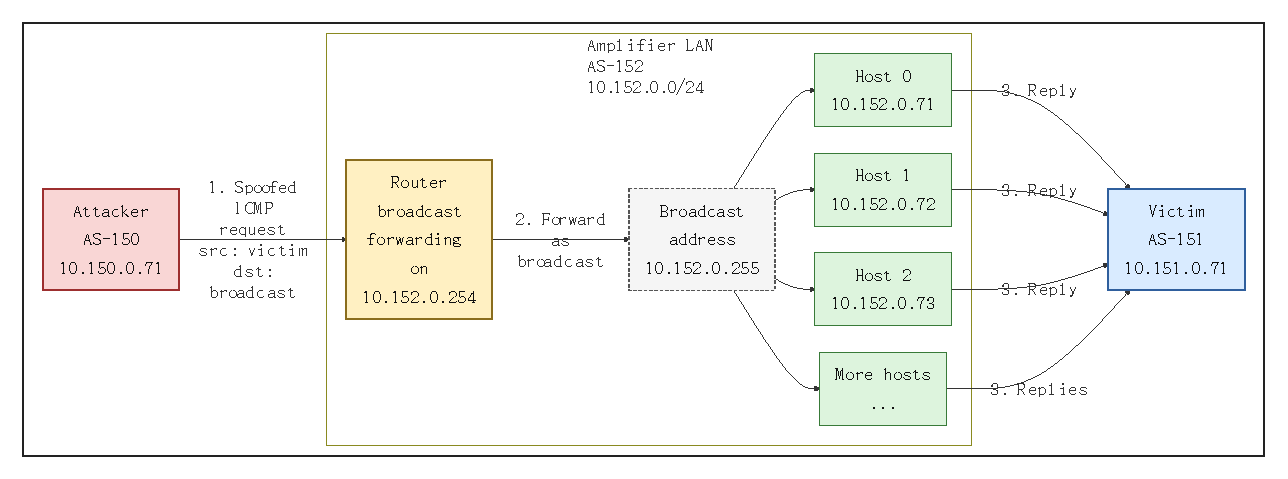
\includegraphics[width=0.95\textwidth]{Figs/smurf_attack.pdf}
\end{center}
\vspace{-0.2in}
\caption{Smurf 攻击}
\label{fig:smurf-attack}
\end{figure}
 

攻击者不需要接收这些响应。主要的可观察效果出现在受害者主机上：受害者会收到
来自许多放大器主机的一批 ICMP echo reply。


\subsection{Fraggle 攻击}

Fraggle 攻击遵循相同的反射模式，但使用 UDP 而不是 ICMP。在模拟器中，放大器
主机在端口 \fraggleport 上运行一个简单的 UDP 响应程序。当它们在该端口收到
UDP 数据包时，会向请求中的源 IP 地址和源 UDP 端口发送响应。

为了让受害者收到被反射的 UDP 响应，攻击者必须把数据包的源 IP 地址伪造成
受害者地址。如果受害者运行 \texttt{nc -ul 7000}，攻击者还应该把 UDP 源端口
设置为 \fraggleport，这样响应才会被交付到受害者正在监听的端口。


\subsection{防御}

可以在多个位置阻止这种攻击模式：

\begin{itemize}[noitemsep]
\item 路由器可以禁用定向广播转发。
\item 主机可以忽略发送到广播地址的 ICMP echo request。
\item 网络可以使用入口/出口过滤，阻止带有伪造源地址的数据包。
\item 服务程序可以避免对较小的未经认证的 UDP 请求发送较大的响应。
\end{itemize}

在本实验中，学生将在模拟器中测试路由器端和主机端的防御机制。


% *******************************************
% SECTION
% *******************************************
\section{实验任务}


% -------------------------------------------
% SUBSECTION
% -------------------------------------------
\subsection{任务 1：检查实验环境}

本任务的目标是熟悉模拟器拓扑，并把观察到的现象与定向广播理论联系起来。

启动模拟器，找到攻击者、受害者、放大器路由器以及若干放大器主机。使用下面的
命令查找并进入相关容器：

\begin{lstlisting}
$ dockps | grep -i attacker   # Attacker
$ dockps | grep -i victim     # Victim
$ dockps | grep -i as152      # Amplifier router and hosts

$ docksh <container-id>       # Enter the container
\end{lstlisting}

在受害者主机上，启动对 ICMP 流量的抓包：

\begin{lstlisting}
# tcpdump -n -i any icmp
\end{lstlisting}

在攻击者主机上，分别 ping 受害者和一台放大器主机。然后尝试 ping AS-152 的
广播地址：

\begin{lstlisting}
# ping -c 3 10.151.0.71
# ping -c 3 10.152.0.71
# ping -c 3 10.152.0.255
\end{lstlisting}

请报告你的观察结果。当使用广播地址时，你看到了多少个响应？第
~\ref{sec:theory} 节中的哪一部分理论可以解释这个现象？


% -------------------------------------------
% SUBSECTION
% -------------------------------------------
\subsection{任务 2：编写 Smurf 攻击程序}

本任务的目标是通过构造伪造的 ICMP 数据包来实现 Smurf 攻击。学生必须在攻击者
主机上使用 Scapy 编写自己的程序。

你的程序应该向 AS-152 的定向广播地址发送 ICMP echo request。该数据包的源 IP
地址应该是受害者的 IP 地址。下面的代码框架展示了程序结构，其中一些重要值被
故意留空。

\begin{lstlisting}[language=python]
#!/usr/bin/env python3
from scapy.all import *

victim_ip = "..."
broadcast_ip = "..."

ip = IP(src=..., dst=...)
icmp = ICMP(type=...)
payload = b"..."

packet = ip/icmp/payload
send(packet, verbose=0)
\end{lstlisting}

你可以在宿主机上使用 vi、gedit 或 vscode 等编辑器编写程序，然后使用
\texttt{"docker copy"} 把程序从宿主机复制到容器中。


在发起攻击之前，在受害者主机上运行 \texttt{tcpdump}：

\begin{lstlisting}
# tcpdump -n -i any icmp
\end{lstlisting}

然后在攻击者主机上运行你的攻击程序。请演示受害者会收到来自多个放大器主机的
ICMP echo reply。在实验报告中，请解释为什么这些响应会发往受害者，而不是发往
攻击者。



% -------------------------------------------
% SUBSECTION
% -------------------------------------------
\subsection{任务 3：测量 Smurf 攻击的放大效果}

本任务的目标是把攻击结果与放大理论联系起来。

修改你的 Smurf 程序，使其发送指定数量的伪造 ICMP echo request，并在数据包之间
加入一个较短的延迟。在受害者主机上，使用 \texttt{tcpdump} 统计收到的 ICMP
echo reply 数量。

\begin{lstlisting}
# tcpdump -n -i any 'icmp and src net 10.152.0.0/24'
\end{lstlisting}

使用不同数量的放大器主机运行实验。如果教师提供了多个版本的模拟器，请比较
结果。如果没有，请记录当前模拟器中的放大器主机数量，并估算预期响应数量。

请在报告中包含以下内容：

\begin{itemize}[noitemsep]
\item 攻击者发送的伪造请求数量。
\item 响应请求的放大器主机数量。
\item 受害者观察到的响应数量。
\item 观察到的结果是否符合放大理论。
\end{itemize}



% -------------------------------------------
% SUBSECTION
% -------------------------------------------
\subsection{任务 4：编写 Fraggle 攻击程序}

本任务的目标是展示相同的反射模式也可以应用于 UDP 流量。

在受害者主机上，使用 \texttt{netcat} 启动一个 UDP 监听器。它会打印交付到
端口 \fraggleport 的 UDP 数据包载荷。

\begin{lstlisting}
# nc -ul 7000
\end{lstlisting}

在攻击者主机上，编写一个 Scapy 程序，把 UDP 数据包发送到 AS-152 的广播地址和
端口 \fraggleport。该数据包的源 IP 地址应该是受害者的 IP 地址。为了让受害者
的 \texttt{netcat} 监听器收到响应，请使用源 UDP 端口 \fraggleport。

\begin{lstlisting}[language=python]
#!/usr/bin/env python3
from scapy.all import *

victim_ip = "..."
broadcast_ip = "..."
port = ...

ip = IP(src=..., dst=...)
udp = UDP(sport=port, dport=port)
payload = b"..."

packet = ip/udp/payload
send(packet, verbose=0)
\end{lstlisting}

请演示受害者会收到来自放大器主机的 UDP 载荷。请解释为什么 UDP 源端口在本任务
中很重要。



% -------------------------------------------
% SUBSECTION
% -------------------------------------------
\subsection{任务 5：防御 1 -- 禁用定向广播}

本任务的目标是测试针对第 3 节所述攻击模式的最直接防御。

进入 AS-152 路由器的 shell，禁用广播转发。不同 Linux 内核暴露这个控制项的
方式略有不同，因此学生应尝试下面的命令，并验证
\texttt{/proc/sys/net/ipv4/conf/} 下的值。

\begin{lstlisting}
# sysctl -w net.ipv4.conf.all.bc_forwarding=0
# sysctl -w net.ipv4.conf.default.bc_forwarding=0
# for f in /proc/sys/net/ipv4/conf/*/bc_forwarding; do echo 0 > $f; done
\end{lstlisting}

再次运行你的 Smurf 和 Fraggle 攻击程序。请报告受害者是否仍然会收到被反射的
流量。请使用定向广播理论解释该防御为什么有效或无效。


% -------------------------------------------
% SUBSECTION
% -------------------------------------------
\subsection{任务 6：防御 2 -- 禁用 ICMP 广播响应}

本任务的目标是测试一种主机端防御，并将其与路由器端防御进行比较。


在每台放大器主机上，配置 Linux，使其忽略发送到广播地址的 ICMP echo request。
由于模拟器可能包含许多放大器主机，我们在 \texttt{Labsetup} 文件夹中提供了一个
脚本，可以把该配置应用到所有 AS-152 主机容器：

\begin{lstlisting}
$ cd Labsetup
$ ./bcast-reply.sh off     # Turn off the broadcast reply 
$ ./bcast-reply.sh on      # Turn on the broadcast reply 
$ ./bcast-reply.sh status  # Show the status
\end{lstlisting}

该脚本会在每个放大器主机容器中运行下面的命令：

\begin{lstlisting}
# sysctl -w net.ipv4.icmp_echo_ignore_broadcasts=1
\end{lstlisting}

再次运行 Smurf 攻击并观察受害者。然后再次运行 Fraggle 攻击。请回答以下问题：

\begin{itemize}[noitemsep]
\item 该防御是否能阻止 Smurf 攻击？
\item 该防御是否能阻止 Fraggle 攻击？
\item 为什么 ICMP 和 UDP 的结果不同？
\item 在本实验中，哪种防御更通用：禁用定向广播，还是禁用 ICMP 广播响应？
\end{itemize}


% *******************************************
% SECTION
% *******************************************
\section{实验指南}

\subsection{运行 Scapy 程序}

伪造原始数据包需要 root 权限。在 SEED 容器内部，shell 通常已经以 root 身份运行，
因此学生可以直接执行 Python 程序：

\begin{lstlisting}
# python3 smurf.py
# python3 fraggle.py
\end{lstlisting}

如果 Scapy 报告权限不足，请确认程序是在攻击者容器内部执行的，而不是在宿主机上
执行的。


\subsection{有用的 Tcpdump 过滤器}

下面的过滤器在本实验中很有用：

\begin{lstlisting}
# tcpdump -n -i any icmp
# tcpdump -n -i any 'icmp and src net 10.152.0.0/24'
# tcpdump -n -i any udp port 7000
# tcpdump -n -i any host 10.151.0.71
\end{lstlisting}

学生应使用 \texttt{-n}，这样 \texttt{tcpdump} 会打印 IP 地址，而不是尝试解析
主机名。


\subsection{检查放大器主机上的 UDP 响应程序}

本实验的 Fraggle 部分使用运行在放大器主机上的一个小型 UDP 响应程序。要检查
它是否正在运行，可以在放大器主机上使用下面的命令：

\begin{lstlisting}
# ps aux | grep fraggle
# tail /var/log/fraggle-amplifier.log
\end{lstlisting}

学生不需要修改该响应程序。攻击程序应写在攻击者主机上。


\subsection{常见问题}

\noindent\textbf{没有观察到被反射的数据包。}
检查攻击数据包中的目的地址和源地址。目的地址应该是广播地址
\texttt{10.152.0.255}；伪造的源地址应该是受害者地址
\texttt{10.151.0.71}。

\paragraph{受害者上的 \texttt{netcat} 没有显示 UDP 载荷。}
请确保在发起 Fraggle 攻击之前已经运行 \texttt{nc -ul 7000}。还要检查你的 UDP
数据包是否使用源端口 \fraggleport；否则，放大器的响应可能会被发送到受害者的
另一个端口。

\paragraph{防御任务似乎没有效果。}
请确认防御命令是在正确的节点上运行的。定向广播转发应在 AS-152 路由器上禁用。
ICMP 广播响应应在放大器主机上禁用。


% *******************************************
% SECTION
% *******************************************
\section{提交要求}

你需要提交一份详细的实验报告，并附上截图，用来说明你完成了什么、观察到了
什么。对于有趣或出乎意料的观察结果，你还需要给出解释。请同时列出重要的代码
片段，并对这些代码进行解释。只提交代码而没有解释将不会获得分数。

此外，请包含以下内容：

\begin{itemize}[noitemsep]
\item 你的 Smurf 和 Fraggle 攻击程序源码，并解释重要的数据包字段。
\item 显示受害者收到被反射 ICMP 响应的截图或终端日志。
\item 显示受害者收到被反射 UDP 载荷的截图或终端日志。
\item 你的放大效果测量结果和解释。
\item 你的防御实验结果，并解释每种防御为什么有效或无效。
\end{itemize}

\end{document}
